\documentclass[10pt]{beamer}

\usetheme[progressbar=head]{metropolis}
\usepackage{appendixnumberbeamer}

\usepackage{booktabs}
\usepackage[scale=2]{ccicons}

\usepackage{pgfplots}
\usepgfplotslibrary{dateplot}

\usepackage{xspace}
\newcommand{\themename}{\textbf{\textsc{metropolis}}\xspace}


\usepackage[utf8]{inputenc} % make weird characters work
\usepackage[english,serbian]{babel}

\definecolor{Teal}{HTML}{004D40}
\definecolor{Orange}{HTML}{FF6D00}

% Theme colors are derived from these two elements
\setbeamercolor{alerted text}{fg=Orange}

% ... however you can of course override styles of all elements
\setbeamercolor{frametitle}{bg=Teal}


\title{Jenkins ukratko}
\subtitle{Sistem za automatizaciju build/test ciklusa}
\date{\today}
\author{Nikola Sojčić, Uroš Milenković, Bojan Nestorović}
\institute{Matematički fakultet, Univerzitet u Beogradu}
\titlegraphic{\hfill
\includegraphics[height=1.5cm]{logo-matf.jpg}}

\begin{document}

\maketitle

\begin{frame}[fragile]{Kontinuirana integracija softvera}
    \begin{itemize}
    	\item Vitalan deo Agilnih metodologija
	\item Nastala kao deo ekstremnog programiranja (eng.~{\em Extreme Programming, XP}) krajem devedesetih
	\item Olakšava upravljanje projektima
	\item Povećava kvalitet koda
    \end{itemize}
\end{frame}

\begin{frame}[fragile]{Kontinuirana integracija softvera -- najbolje prakse}
    \begin{itemize}
    	\item Jedinstveno skladište za kod
	\item Automatizacija izgradnje i testiranje softvera
	\item Održava izgradnju softvera brzom
	\item Svaki programer objedinjuje kod svakodnevno
	\item Svako može da vidi šta se dešava
	\item Automatsko objavljivanje novih verzija softvera
    \end{itemize}
\end{frame}

\begin{frame}{Kontinuirana integracija softvera -- dijagram}
  \begin{figure}
    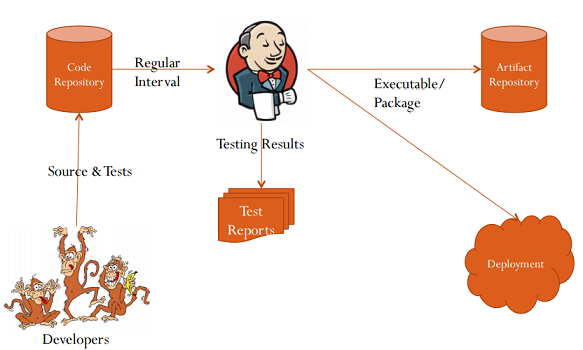
\includegraphics[scale=0.55]{workflow.png}
    \caption{Kontinuirana integracija softvera}
  \end{figure}
\end{frame}

\begin{frame}[fragile]{Posao izgradnje}
  \begin{itemize}
            \item Kreiranje posla izgradnje
            \item Integracija sa sistemom za kontrolu verzija
            \item Pokretanje izgradnje
			\item Koraci izgradnje
            \item Akcije posle izgradnje
  \end{itemize}
\end{frame}

\begin{frame}[fragile]{Integracija sa sistemom za kontrolu verzija}
  \begin{itemize}
            \item Subversion
            \item CVS
            \item Git - \alert{\emph{mora se instalirati dodatak}}
			\item i ostali
  \end{itemize}            
\end{frame}

\begin{frame}[fragile]{Pokretanje izgradnje}
  \begin{itemize}
            \item Build periodically - pokretanje u određenom vremenskom intervalu
            \item Poll SCM - pokretanje posle promena izvornog koda
            \item Build after other projects are built - pokretanje izgradnje nakon pokretanja druge izgradnje
  \end{itemize}
\end{frame}

\begin{frame}[fragile]{Automatsko testiranje}

        
        \begin{itemize}
            \item Bitna aktivnost u ciklusu \cite{jenkins:2011}
            \item Razvoj vođen testovima (eng.~{\em Test Driven Development})
            \item Testovi jedinica (eng.~{\em Unit tests})\cite{docs:unit}
            \begin{itemize}
                \item JUnit
                \item \alert{\emph{x}Unit}
            \end{itemize}
            \item Standardizovan \texttt{XML} izveštaj za testove jedinica
        \end{itemize}

\end{frame}
\begin{frame}[fragile]{Uključivanje testova jedinica u proces}    
      Prikazivanje rezultata testova
      \begin{enumerate}
        \item Dodati novu ``post--build akciju``
        \item Izabrati ``Publish JUnit test result report`` 
        \item Upisati putanju do \texttt{XML} izveštaja u ``Test report XMLs``
        \item Pogledati grafikone na početnoj strani
      \end{enumerate}
\end{frame}

\begin{frame}[fragile]{Pokrivenost koda}
    \begin{itemize}
        \item Metrika koja se ceni u testiranju softvera
        \item Ne daje značajnu informaciju o kvalitetu napisanog koda već koliki deo koda je pokriven testovima jedinica
        \item Cobertura za Javu
        \item Neki alati za \emph{x}Unit testove imaju ugrađene sisteme za pokrivenost koda 
        \begin{itemize}
            \item Dodaci su uglavnom pametni da mogu da prepoznaju ugrađene sisteme i da ih konfigurišu za Jenkins
        \end{itemize}
    \end{itemize}
\end{frame}

\begin{frame}[fragile]{Automatsko objavljivanje novih verzija softvera}
    \begin{itemize}
	\item Glavni posao je da omogući da ceo proces prodje nesmetano i automatski
	\item Kod se posle završenog posla šalje na server spreman za krajnje korisnike
	\begin{figure}
	    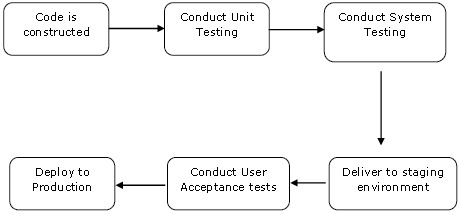
\includegraphics[scale=0.55]{slika2.jpg}
	    \caption{Proces automatskog objavljivanja}
	\end{figure}
    \end{itemize}
\end{frame}

\begin{frame}[allowframebreaks]{Reference}

  \bibliography{demo}
  \bibliographystyle{abbrv}

\end{frame}

\end{document}
